\chapter{Background}
This chapter introduces the necessary background information needed for understanding the rest of the report.
First section, provides a broad introduction to \ac{sdr} systems, GNU Radio Software Tool and \ac{PHY} and \ac{mac} layers of the network stack.
The second section introduces the LimeSDR platform and its hardware and software architecture.
Wime Project and IEEE 802.15.4 is explained in the third section.
Finally, the fourth section introduces the tools used in the methods chapter.


\section{Essential Concepts}
\subsection{\ac{PHY} and \ac{mac} Layers}
\ac{OSI} Model (ISO/IEC 7498-1:1994) presents the abstract model for networking, that is used for most communication systems design.
The abstract model is divided into 7 layers,  where entity in each layer implements the functionality of the layer and interacts directly with the layer beneath it.
This added functionality can be used by the upper layers.
Data from the user application is encapsulated by each subsequent layers of the \ac{OSI} model into their frame format.
These frames carry meta-data in the form of frame headers.
Different protocols use different frame format and headers  as it helps differentiate one protocol from another.
These headers help the receiver in learning where the incoming data packet is coming from, who is it meant for, how to decode and arrange the contents of the data packets etc.\\

The \ac{PHY} layer is the lowest layer (L1) of the \ac{OSI} model,it interacts with the physical communication channel directly.
It specifies the type of data transfer(serial/parallel) and data rate of the protocol.
The \ac{PHY} layer defines the process of transmitting raw bits through the physical medium.
The bit-stream is grouped into code words and converted to symbols, which are then modulated to a physical signal for transmission over the transmission medium.
\ac{PHY} layers also provides physical transmission link information like carrier sense, collision detection and \ac{LQI}  to the upper layers. \\


\ac{mac} layer, \ac{L2} of the \ac{OSI} model, is responsible for defining the methods for sharing and using the common transmission medium among multiple devices.
%\ac{mac} layer addresses are used to to check if the incoming packet is meant for the device.
In case of outgoing packets, the \ac{mac} layer adds the \ac{mac} address of the destination device to the packet header.
It adds the synchronization preamble and \ac{FCS} for checking transmission error.
Retransmission in case of dropped packets and acknowledgement to successfully received packets are handled by this layer.\\

\begin{figure}[h!]
\centering
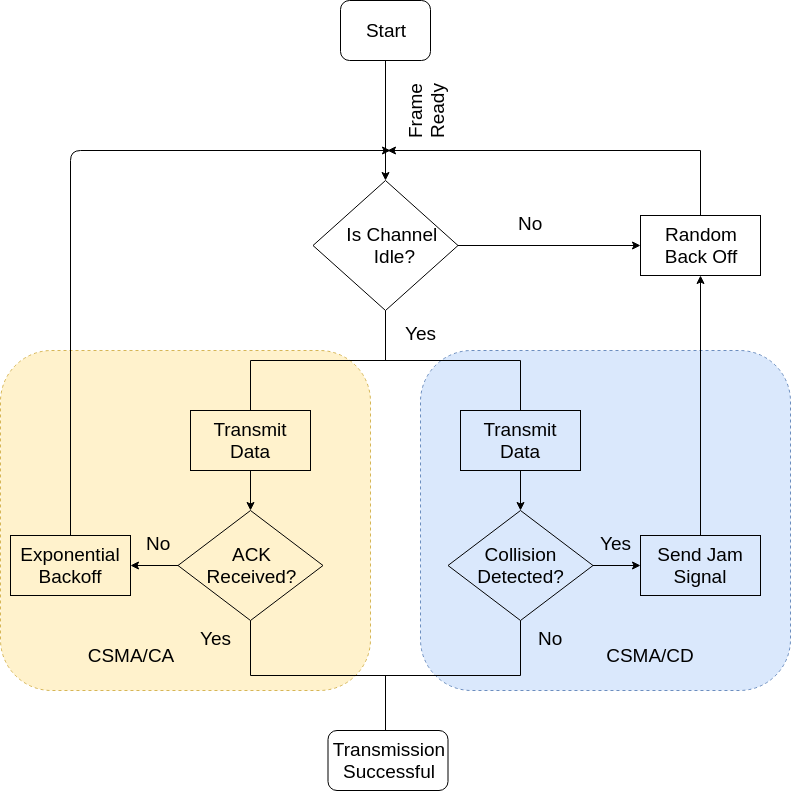
\includegraphics[width=0.9\textwidth]{Figure/CSMA.png}
\caption{CSMA flow graph.}
\label{Csma_flow}
\end{figure}

\ac{csma} is a \ac{L2} protocol in the OSI Model. 
%It is a method for handling multiple access of a shared medium.
It mainly comes in two varieties: \ac{CSMA/CD}  and \ac{CSMA/CA}.
The flow graphs of both are shown in Figure \ref{Csma_flow}.
In the older \ac{CSMA/CD}, the nodes checks the idleness of the channel after the frame is ready.
If idle it starts transmission.
During transmission, it monitors the medium for collision.
If collision is detected, it employs a collision recovery process, where it sends a jam signal to signal other nodes that a collision has occurred.
Then it waits for a  random delay and starts transmission again.\\

\ac{CSMA/CA} tries to avoid collision, it starts off similar to \ac{CSMA/CD} where it senses to check when the channel is idle.
If found idle, it starts transmission.
It is difficult for wireless nodes to detect collisions simultaneously during transmission.
Therefore, it relies on an \ac{ack} message from the receiving node to check if the data packet was received.
If \ac{ack} is not received, the node assumes a collision has occurred and  uses exponential back-off to determine when the next time to re initiate transmission.\\


\ac{tdma} is also a \ac{L2} protocol, where a coordinator schedules medium access to the nodes in a periodic manner.
Communication happens in time-slots.
Each node in the network is given exclusive access to transmit during its time slot.
The coordinator generates beacon signals periodically to maintain relative time synchronization. On receiving the beacons, the nodes adjust their transmit clocks so that they have the correct estimate of their time-slots.
 
 

\subsection{\ac{sdr} Platforms}

\ac{sdr} presents a new paradigm of communication system design where the system is flexible to adapt to the needs of the end-user as also the radio channel conditions. Nychis et.al \cite{nychis_enabling_nodate} classifies \ac{sdr} based communication systems into two main architectures.
\begin{itemize} 
\item{\textit{Host-PHY Architecture:} This is the most common architecture, enabling design and development of the entire system in software.
It provides the maximum flexibility in terms of design and implementation choices, also there is added benefit of easy upgrades.
But, since the system is designed is software only, the processing and communication delays make most modern \ac{mac} protocols infeasible in this architecture.}


\item{\textit{NIC-PHY Architecture:} In this architecture most of the \ac{PHY} layer functionality is implemented in \ac{FPGA} and \ac{DSP}.
The closer proximity to the radio hardware and specialized parallel hardware processing makes this architecture most suitable for running the modern \ac{mac} protocols.
But the design process for this architecture based systems is time consuming and difficult, as traditionally hardware programming is harder than software programming.
However, they are much more flexible compared to commercial \ac{NIC}.
\textit{Wireless Open Access Research Platform}(WARP) \cite{noauthor_warp_nodate} is an example of system based on this type of architecture.}

\end{itemize}
Since host-PHY \cite{nychis_enabling_nodate} is the most commonly used architecture (\textbf{cite sources}), the report concentrates on explaining the functionality of \ac{sdr} systems using this architecture.
Figure \ref{host_PHY} shows the typical design of communication systems in this architecture. The system can be broadly divided into two main components:
\begin{enumerate}
\item{\ac{sdr} Platform.}
\item{Host Computer.}
\end{enumerate}

\begin{figure}[h!]
\centering
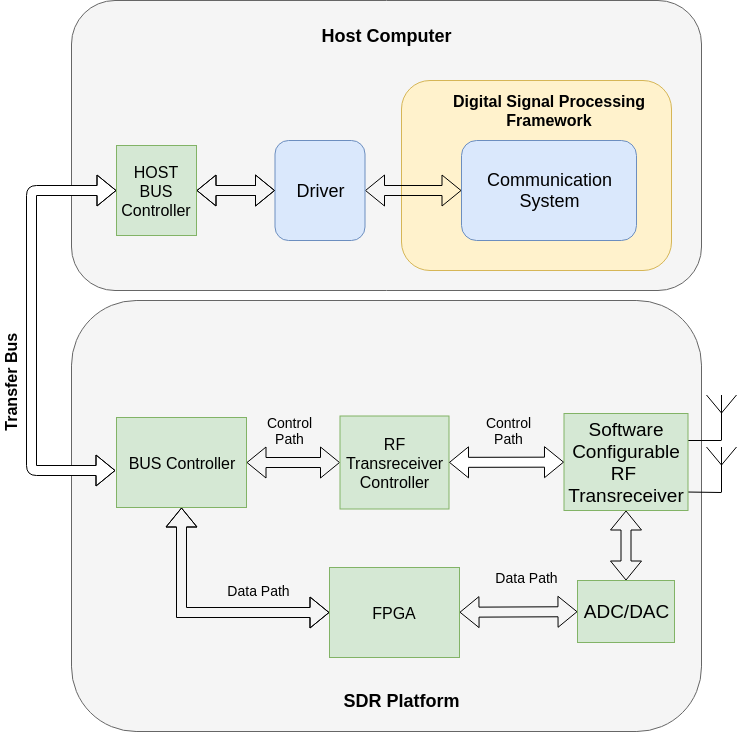
\includegraphics[width=\textwidth]{Figure/Host_Phy.png}
\caption{Host-PHY \cite{nychis_enabling_nodate} \ac{sdr} architecture.}
\label{host_PHY}
\end{figure}


Since the process for transmission and reception processes are reverse of one another , this report concentrates on the explaining the reception process of \ac{sdr} platforms.

\paragraph{\ac{sdr} Platform:} It is the hardware that provides access to the wireless medium in a flexible manner.
\ac{RF} signals are transmitted and received by the platform, it converts these analog signals to digital samples and transfers them to the host computer.
The main building blocks of these platforms are shown in Figure \ref{host_PHY}.
\begin{itemize}
\item{\textbf{Software Configurable \ac{RF} trans-receiver}} This is the heart of \ac{sdr} platforms and provides \ac{RF} modulation and demodulation capability.
They are attached to wide-band antennas for receiving and transmitting over a broad range of frequencies.
Taking the case of reception of RF signal, the signal received from the antenna is amplified by a \ac{LNA}.
The \ac{LNA} amplifies a low power signal without significantly degrading the signal to noise ratio.
Once amplified, the signal is passed to a \ac{RF} receiver, where the \ac{RF} signal is demodulated either to an intermediate frequency or baseband signal depending on whether the the receiver is a Zero-IF receiver or Super-heterodyne receiver respectively.\\

\begin{figure}[h!]
\centering
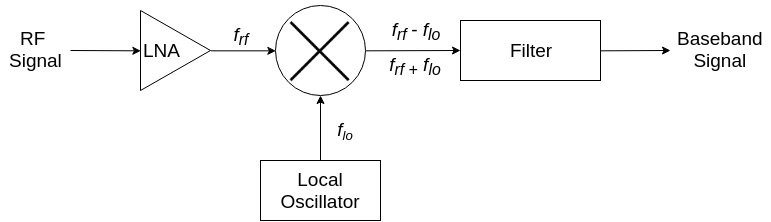
\includegraphics[width=0.8\textwidth]{Figure/RF_receiver.png}
\caption{Simple \ac{RF} receiver.}
\label{rf_receiver}
\end{figure}

Figure \ref{rf_receiver} shows a simple \ac{RF} receiver in which the \ac{LNA} output signal is fed to a mixer.
The mixer is a signal processing block used for translating the input signal to another frequency range.
The mixer uses a locally generated carrier frequency for the translation. 
If the input \ac{RF} signal has a frequency of $f_{rf}$, and the local oscillator frequency is $f_{lo}$ then the mixer will produce a signal with frequency components $f_{rf}-f_{lo}$ and $f_{rf}+f_{lo}$.
This output signal is then passed through a band-pass filter with $f_{rf}-f_{lo}$ as center frequency, this will reject the unwanted $f_{rf}+f_{lo}$.
If we assume $f_{rf}=f_{lo}$, the bandpass filter will be equivalent to a low pass filter and the output signal will be the baseband signal.
This is the case in Zero-IF receiver architecture.
In super heterodyne receiver architecture, a number of intermediate frequency stages are used before generation of the baseband signal.\\

In traditional trans-receiver, a crystal oscillator is used.
This results in good stability of the local oscillator signal but the system is now tuned to a particular frequency.
With the goal of flexibility in mind, \ac{sdr} platforms use frequency synthesizers to generate the local clock signal.
Frequency synthesizers are used for creating arbitrary waveforms from a single frequency clock.
Most \ac{sdr} use \ac{DDS} as the frequency synthesizer, which uses a highly stable oscillator used as a reference signal.



\begin{figure}[h!]
\centering
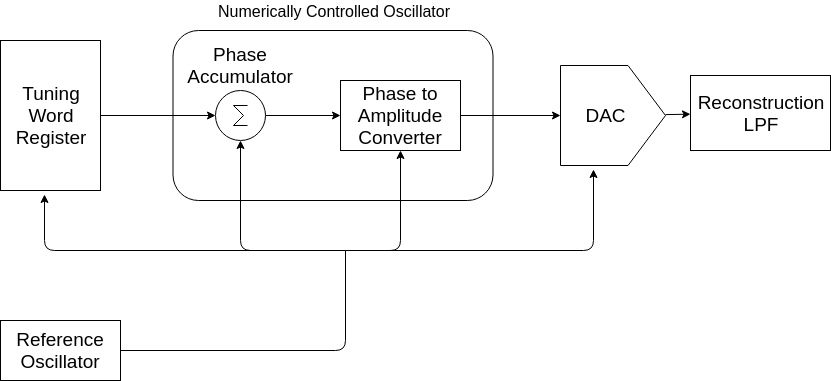
\includegraphics[width=0.8\textwidth]{Figure/DDS.png}
\caption{DDS}
\label{dds}
\end{figure}

The main components of a \ac{DDS} are \ac{NCO} which is made of the Phase Accumulator and Phase to Amplitude Converter, \ac{DAC} and a Tuning Word Register as shown in Figure \ref{dds}.

In each clock cycle, the phase accumulator increases the output(phase) by the value stored in the Tuning Word Register.
This output is the input to the Phase to Amplitude Converter, which basically is a lookup table containing the amplitude for a particular phase.
The output of the Phase Accumulator is basically the address(phase) for the lookup table.
The output is then converted to an analog signal by the the \ac{DAC} and then passed through a low pass filter to smoothen out the waveform.

Since the Tuning Word Register is responsible for how fast the phase changes, the output sinusoid frequency can be controlled by controlling the Tuning Word Register, this is how \ac{sdr} platforms are able to generate a wide range of local oscillator frequencies.

In \ac{sdr} platforms, the filter (shown in Figure \ref{sdr_architecture} is implemented using \ac{FIR} filters.
\ac{FIR} filters are convolutional filters where the output response of a particular input is finite.
The output of a \ac{FIR} filter can be adjusted by readjusting the parameters of the filter's impulse response.
This allows for the \ac{sdr} to allow certain range of frequencies in the output, which can be adjusted by external control.

\item{\textbf{\ac{RF} Trans receiver Controller:} The controller provides the interface to control the \ac{RF} Transceiver.
The communication system running on the host computer, provides the desired RF parameters to the controller.
It then translates those instructions to digital signals for configuring the RF trans-receiver modules like the \ac{FIR} filter weights, the tunable word register for selecting the desired frequency and also the desired gain in the programmable gain amplifiers.
}

\item{\textbf{ADC/DAC:} The filtered analog \ac{RF} signal needs to be converted to digital domain before transferring to the host computer.
Fast data converters are used on the \ac{sdr} platforms for this purpose.
The sampling rate of these data converters determine the available \ac{RF} bandwidth of the system according to the Nyquist criteria.
The resolution of the \ac{sdr} data converters are important so as to ensure high dynamic range of the received signal, ensuring that the system is capable is receiving very weak signals as well very strong signals without saturation.
The sampling rate of these data converters are controlled by the \ac{RF} trans-receiver controller.
}
\item{\textbf{\ac{FPGA}:} The \ac{FPGA} provides acts as the glue logic between the data converters and the bus controller.
In most cases the bus communication is bursty in nature, whereas the \ac{DAC} produces a stream of samples.
\ac{FPGA} provides for efficient buffering of these samples, packs them into bursts to be sent over the bus.
In some platforms, additional information like a sample clock is also packed into these bursts.
Some applications might need additional signal processing, \ac{FPGA} provides for a efficient way for implementing these filters.
In NIC-PHY architecture most of the communication system is designed using the \ac{FPGA}.
}
\item{\textbf{Bus Controller:} It is the bridge for the bursts of data crossing over from the \ac{sdr} platform to the host computer and vice versa.
It takes in data packets from the \ac{FPGA} encodes them with bus transfer protocol, then initiates transfer.
The flow control and routing for different packets is also handled by the bus controller.}
\end{itemize}

\paragraph{Host Computer:} The host computer, a general purpose computer, is the brain of the communication system.
It runs the software implementation of the baseband processing for the desired protocol, taking the digital samples from the \ac{sdr} as input.
During initialization, it configures the \ac{sdr} platform.
Depending on implementation, it can have the full network stack and an application running on top of it.
From architectural viewpoint, the host computer has three main components as shown in Figure \ref{host_PHY}.

\begin{itemize}
\item{\textbf{Bus Controller:} The bus controller on the host computer controls the other end of the bus communication link.
It decodes the received data bursts and sends them to the driver for further processing.
If the bus communication involves a master slave relationship, then the host computer bus controller is designated as the master.
It initiates the data transfer on the bus, and the slave bus controller  responds to the requests placed by this bus controller.
}
\item{\textbf{Driver:} The driver is the abstraction layer for the \ac{sdr} platform communication and configuration.
The communication system designer should be able to provide high level instructions to the \ac{sdr} platform.
It is left to the driver to handle the translation of high level instructions to low level register control data words.
For example, when tuning the RF trans-receiver, the system designer would be much more comfortable to say set the center frequency to 1.8 GHz, rather than saying set register at address "x" to value "data".
The driver handles this translation.
It also is responsible for ensuring a reliable data transfer link.
Since the communication system and the incoming data may be running at different rates, the driver buffers the incoming data and provides it to the the running communication system at its data processing rate.}
\item{\textbf{Digital Signal Processing Framework:} The hardware baseband processing of communication systems are generally designed with concurrent execution in mind.
Whereas, general purpose computing platform are sequential in nature. Many core processors add the capability of concurrent execution but at a much smaller scale than what can be acheived with hardware processing platforms like \ac{FPGA} and \ac{ASIC}.
So when designing systems on general purpose computing platforms, this change in execution model needs to be taken into account.\\

Threads provide a software method to implement concurrent execution model. 
But, efficient thread management and synchronization produces significant overhead.
Digital Signal Processing frameworks are designed to help system designers to only design their signal processing modules without worrying about thread synchronization and management.
They are designed with concurrent execution of signal processing algorithms and modularity of system design in mind.
Two of the most popular frameworks are GNURadio and Labview.
In the next section, the report goes into detail about GNU Radio. 
}
\end{itemize}
\subsection{GNU Radio}

GNU Radio is an open-source digital signal processing framework, which has been rapidly evolving with a large active community.
The software framework can be used for both simulation and prototyping real-world application scenarios. 
It  provides a graphical interface for designing signal processing chains  as well as extensive library of signal processing blocks like filters, synchronizers, demodulators etc.
The ease of use of the framework, extensive library as well as hardware support for most \ac{sdr} platforms has led to diverse application use cases such as RFID, 802.11, cellular networks.\\


GNU Radio is designed to stream large amounts of data in real-time between parallel computational nodes.
The data flow between the nodes from the source to the sink is described by the flow-graph, while the flow of data is controlled by the GNU Radio Scheduler.
Figure \ref{gnuradio_arch}, shows a simple flowgraph where the data from the Sources node is processed by the signal processing chain.
The processed data is sent to the Sink nodes.
The signal processing chain itself is composed of multiple data processing nodes, for example the flow graph in Figure \ref{gnuradio_arch} has 4 nodes in the processing chain.
The scheduler is in task of scheduling the execution of these blocks. 
From the block designer point of view, these blocks can be viewed to be executing concurrently.

\begin{figure}[h!]
\centering
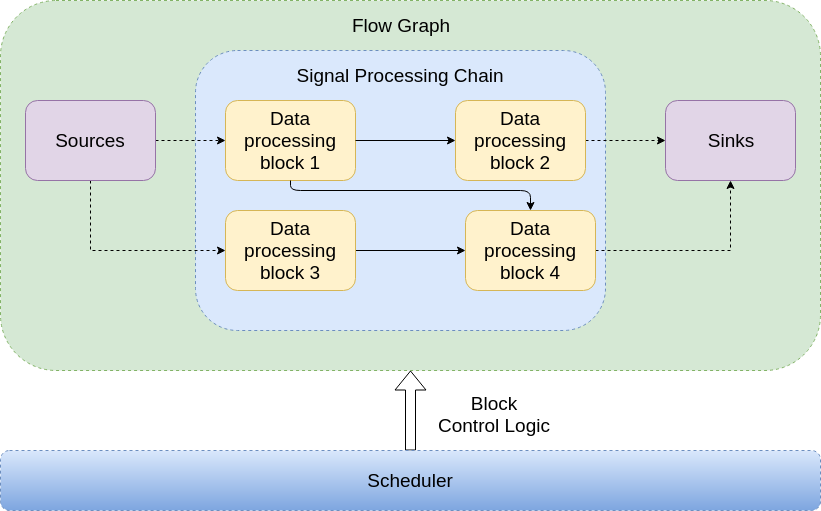
\includegraphics[width=0.9\textwidth]{Figure/GNURADIO_1.png}
\caption{GNU Radio Software Architecture.}
\label{gnuradio_arch}
\end{figure}

\paragraph{Blocks and Flow Graphs}

The computational nodes in the flow-graph are the GNU Radio processing blocks.
Each block describes how the input elements to the block, are converted to output elements in the \textit{work} function.

\begin{table}[h!]
\centering
\begin{tabular}{|c|c|c|}
\hline
Number of input elements & Number of output elements & Name\\
\hline
N & 0 & Sink Block\\
0 & N & Source Block\\
N & 1 & Interpolation block\\
1 & N & Decimation block\\
M & N & General Block\\
\hline
\end{tabular}
\caption{GNU Radio Block Types}
\label{block_type}
\end{table} 

The relationship of input and output elements defines the type of the GNU Radio processing block as shown in Table \ref{block_type}.
The type of block indicates the scheduler on how the block processes information.
There are two types of blocks: \textit{Synchronous block} and \textit{block}.
For synchronous blocks, there is a rational relationship between the input and output elements.
The sink, source, interpolation block and decimation block in Table \ref{block_type} are synchronous blocks.
The key difference between different block types is in how the scheduler handles the input and output buffers of each block.
For the synchronous blocks, the scheduler implicitly handles the input and output pointers to the buffers.
For general blocks, the \textit{work} function needs to explicitly pass the information on how many elements it consumed and produced.\\

Since in GNU Radio flow graph, data is passed from one node to another, the method of passing the data among different blocks needs to be defined.
This method is defined in the block interfaces.
Stream Interfaces are intended to stream large amounts of data between blocks with variable processing rates.
They use large buffers to pass the data from one node to another.
Stream interfaces work well for samples, bits etc. but they are not the right method to pass metadata, control information or bursts of data between blocks as it involves significant overhead.\\

GNU Radio recently added the message passing interface for handling asynchronous message passing.
GNU Radio also supports stream tags for handling metadata as it is closely associated with the stream data samples.
Stream tags are attached with stream data samples and provide additional information associated with the sample.
It can be used both for passing control flags as well as metadata information like the \ac{PDU} size, timing information etc.
These stream tags are propagated to the next blocks and is updated by the data rate changes.
For example, if the block takes it 2 samples as input and produces 4 samples as output, its data rate is 2.
In this case, if the input stream had a stream tag at position "x" then the the location in the output stream would be "2x". \\


\begin{figure}[h!]
\centering
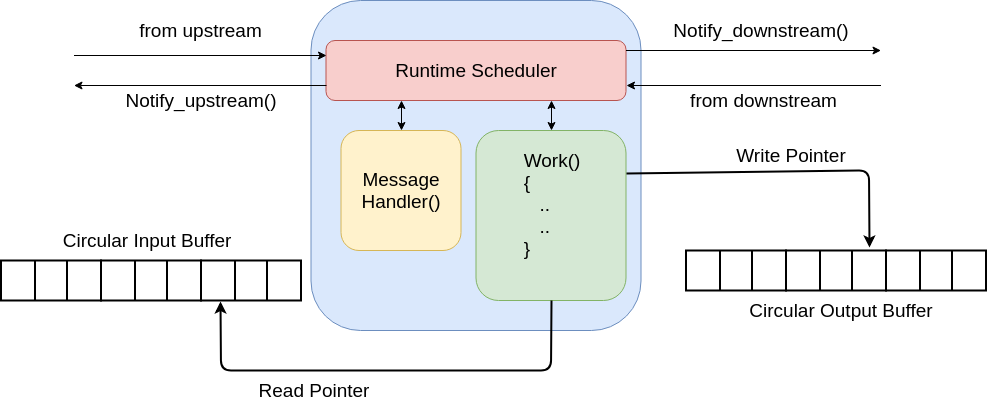
\includegraphics[width=0.9\textwidth]{Figure/Block.png}
\caption{Architecture of GNU Radio block}
\label{block_arch}
\end{figure}

Figure \ref{block_arch} shows the general architecture of a GNU Radio block. 
Each block has associated buffers for the stream interfaces, two computational components, namely the \textit{work} function and the \textit{message handler} function.
A run time scheduler is associated with each block for controlling the execution of block during runtime. The runtime scheduler has its own signaling mechanism for interacting with schedulers of other blocks.
This signaling mechanisms are hidden to the flow graph designer, and are used for flow control.
The blocks providing the inputs to the current block are called upstream blocks, while those that are fed by the output of this block are called downstream block.\\

For the sake of simplicity, it is assumed that the current block in Figure \ref{block_arch} has one upstream block and one downstream block.
This implies that the block has a single input buffer and a single output buffer.
The \textit{work} function describes the implementation of the signal processing algorithm.
On starting execution, the \textit{work} function accesses data from the circular input buffer, which is same as the output buffer for the upstream block.
Both the upstream block and the current blocks maintains a pointer to the last used data element position. 
Once completion of execution, the upstream block writes new elements to the input buffer of the current block and updates its the write data pointer.
The upstream block notifies the current block using the notify\_ downstream() method that new input data elements have been written.
The scheduler for the current block checks if there is sufficient new data for a single execution.
It then starts the execution of the current block once the input buffer has sufficient data.
On successful execution, it updates the read data pointer, writes the data elements into the output buffer and updates the write pointer.\\

Since, most filter design rely on history of previous inputs, the scheduler also notifies the upstream block on reading the data from the buffer to notify that its output might have been modified.
The current block scheduler notifies the downstream block that new data elements are available when it writes to the output buffer.
The \textit{message handler} function works similarly, in this case the upstream block scheduler uses notify\_msg() method for signaling that a new message may be available.\\

The flow graph describes the flow of data between different blocks.
Flow graphs make it easier to design complex signal processing algorithms by combining simpler blocks.
This provides modularity and scalability to the algorithm development process.
Generally blocks are designed in C++ to enable fine grained control and faster execution.
Python's QT framework defines a signals and slot mechanism for communicating events between different objects.
Slots are instantiation of C++ objects, which in this case are the the processing blocks.
When the internal state of the block is changed, it emits a signal which notifies other slots an event has occurred.
This mechanism is used for describing the flow graphs.


\paragraph{Scheduler}
The scheduler is the control unit for the flow graph.
At initialization, the scheduler allocates the buffers and instantiates each block in its own thread.
At runtime, it does memory management for each block, determines the requirements that are set by the block such as number of items to be processed in one execution, alignment of data in the buffers etc.
Once the requirements are satisfied, it passes the read and write pointers to the \textit{work} function and starts the one execution.
Once the \textit{work} function finishes its execution, the scheduler takes in the returned information and updates the state of the block and the appropriate pointers.\\


\section{LimeSDR-USB}
The \ac{sdr} platform used in this project is LimeSDR-USB.
It follows the architecture of the \ac{sdr} platform shown in Figure \ref{host_PHY}.
The technical specifications of LimeSDR-USB and the component description in reference to Figure \ref{host_PHY} has been summarized in Table \ref{specs}.
In the next subsections, the report discusses the hardware and software architecture of LimeSDR-USB.


\begin{table}[h!]
\centering
\begin{tabular}{|c|c|}
\hline
Feature & Description\\
\hline
Software Configurable RF Transreceiver & LMS7002 MIMO \ac{FPRF}\\
\ac{FPGA} & Altera Cyclone IV EP4CE40F23 \\
Bus Controller & Cypress USB 3.0 CYUSB3014-BZXC\\

\hline
\end{tabular}
\caption{LimeSDR-USB specifications}
\label{specs}
\end{table}

\subsection{LimeSDR-USB Hardware Architecture}

\begin{figure}[h!]
\centering
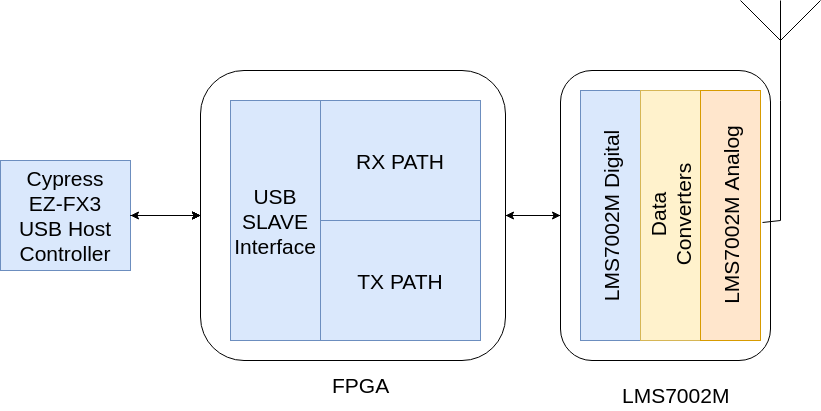
\includegraphics[width=0.9\textwidth]{Figure/Lime_Hardware.png}
\caption{Block Diagram of LimeSDR-USB.}
\label{lime_hw_arch}
\end{figure}

Figure \ref{lime_hw_arch} shows the block diagram of a LimeSDR-USB board.
For the sake of simplicity the diagram shows the major components, namely the LMS7002M \ac{FPRF}, \ac{FPGA} and the Cypress FX3 Bus Controller.
Other components will be introduced in correspondence to their application with these major components.

\subsubsection{LMS7002M} 

LMS7002M is a fully intergarted \ac{FPRF} transreceiver providing 2$\times$2 \ac{MIMO} functionality.
It provides continuous coverage in the 100kHZ- 3.8GHz frequency range, with on chip data converters providing 160 MHz \ac{RF} bandwidth.
It is designed for a broad range of applications, ranging from broadband wireless communication, cellular communications, \ac{sdr} applications etc.
The hardware mainly consists of three main sub-components: analog processing chain, data converters and digital processing chain.\\

\begin{figure}[h!]
\centering
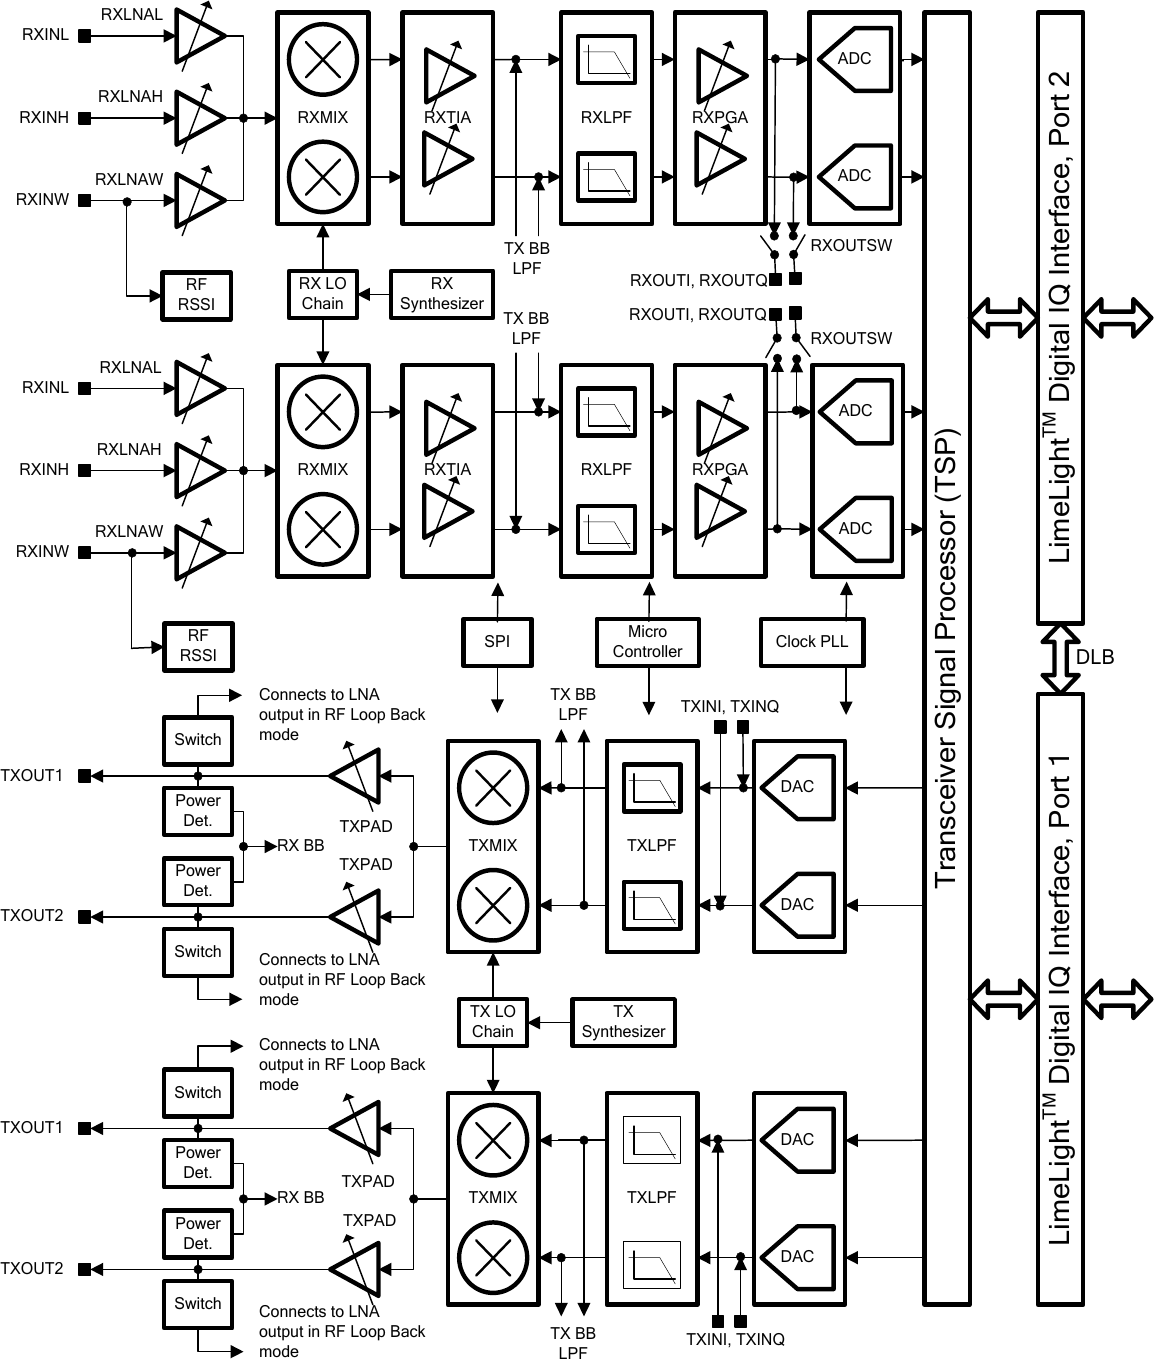
\includegraphics[width=0.9\textwidth]{Figure/Lms7002m-block-diagram.png}
\caption{Block Diagram of LMS7002M.}
\label{lms7002m}
\end{figure}

LMS7002M offers full duplex communication link on both the TX and RX chains.
Each of the RX chains has three separate \ac{RF} ports tuned for narrow band low frequency, narrow band high frequency and wide band operations.
Similarly, the TX Chains are connected two separate \ac{RF} ports tuned for high frequency and low frequency operations.
This separation is done for better impedance matching at the boundary of the antennas.\\

Figure \ref{lms7002m} shows the functional block diagram for a LMS7002M \ac{FPRF}.
Since, both the RX and TX paths are identical, the report concentrates on only one RX path.
The output from the \ac{RF} RX ports are fed into the \ac{LNA} inorder to minimize injecting too much noise at the beginning of the chain.
The receiver follows the architecture shown in Figure \ref{rf_receiver}, with a RX mixer, followed by filter and a \ac{PGA} combined in a Zero-IF architecture.
The RX \ac{PGA} outputs the analog baseband signal.\\

LMS7002M uses a fractional N-\ac{PLL} architecture for the local oscillator frequency synthesis.
\ac{PLL} is used extensively in \ac{RF} circuits for making sure the generated local oscillator signal and the reference signal have the same phase and frequency.
PLLs are essentially negative feedback systems, so when the input signal differs a lot from the output signal, the control logic tries to lower the error (\textit{input-output)}.\\

Integer N- \ac{PLL} architectures are used to generate high frequency signals from low frequency reference clocks, by using a frequency divider in the negative loopback path.
The frequency divider is basically a counter, that outputs every "N" (division factor of the loop) clock cycles of the output signal.
But since the output signal frequency will be multiples of the reference clock, the output signal resolution is determined by the  reference clock.\\

So to have a high frequency as well as a high resolution, the divider counter should be very large in size.
To counter the problem, fractional N-{PLL} architectures were designed where the output signal frequency can also be a fractional multiple of the input signal frequency.
This helps in increasing the frequency resolution without the need for a large divisor counter.
The input and output frequency relationship for a fractional  N-\ac{PLL} can be summarized by: $f_{out}=f_{ref}(N+k/M)$, where N is the integer divider factor, k is the fractional divider factor and $1/M$ gives the output frequency resolution.
Both the integer and fractional divider factor are determined by the size of the counters used.
In case of LimeSDR, the reference signal fed to the PLL varies from to 10 to 52 MHz.
The output signal can vary from 30 to 3800 MHz, with a frequency resolution of 24.8 Hz.\\

Once the \ac{RF} demodulation is completed by the analog processing chain, the analog signal is sent to the data converters and converted to digital data samples.
The sampling rate for the data conversion is determined by the required \ac{RF} channel bandwidth.
The digital samples are sent to the \ac{TSP} for further processing.\\

The \ac{TSP} uses advanced signal processing algorithms like IQ DC offset correction, IQ phase correction for correcting the received samples.
An interpolation and decimation filter is added to the \ac{TSP} for the TX and RX chains respectively.
These filters are implemented with a chain of five fixed co-efficient half band \ac{FIR} filters, which allows interpolation and decimation factors of 1,2,4,8,16.
Interpolation and Decimation allows the baseband to run at a lower data rate while still running the data converters at higher sampling rates, enabling the quantization noise to be spread over larger frequency range.
Automatic Gain Control is also implemented by the the \ac{TSP}.\\


LMS7002M interfaces can be segmented into control interfaces and data interfaces.
The control interfaces are used for initialization, calibration and on the fly reconfiguration of the LMS7002M parameters.
The data interface is used for exchanging \ac{IQ} samples with the baseband modem.
For the data interface, LMS7002M uses the LimeLight interface which implements a 12 bit JESD \ac{DDR} interface for each RX/TX chain as shown in Figure \ref{lms7002m}.
The LMS7002M has a on-chip micro-controller which can be used for configuration and control of the LMS7002M chip.
It also provides a \ac{SPI} interface for offloading the control and configuration functionality to the baseband modem.


\subsubsection{FPGA}

The LMS7002M is designed to stream data continuously, whereas the Cypress FX3 uses USB 3.0 protocol transmits packets of data.
LimeSDR-USB uses an Altera Cyclone IV \ac{FPGA} to buffer the streaming data, converts them to packets and adds meta-data to each packet as recommended by Nychis et.al \cite{nychis_enabling_nodate}.
The architecture of the FPGA data path blocks is shown in Figure \ref{lime_hw_arch}.
The TX path is responsible for moving data from the USB interface to the LMS7002.
The RX Path on the other hand controls the reception of samples from the LMS7002M and subsequent sending to the Host-Computer via the USB interface.
The \ac{FPGA} also has on board PLLs which are configured to be the same as the sample clock\\

The \ac{FPGA} interfaces are designed to handle the segregation of control and data paths by LMS7002M.
The data paths (TX path and RX path) uses a 12-bit parallel interface to stream data to and from the LimeLight interface of the LMS7002M.
The control path of the \ac{FPGA} has a NIOS processor which interacts directly with the USB Slave Interface and controls the \ac{RF} parameters through an \ac{SPI} interface.\\

The \ac{FPGA} RX path converts samples to packets which takes significant buffering time.
As this report concentrates on study of timing delays, it is necessary to take a closer look at the \ac{FPGA} implementation and understand the buffering process.
In contrast, \ac{FPGA} TX path converts packets to samples and there is no need for buffering.
So in the next paragraph, the report describes the \ac{FPGA} RX path in detail.
 

\begin{figure}[h!]
\centering
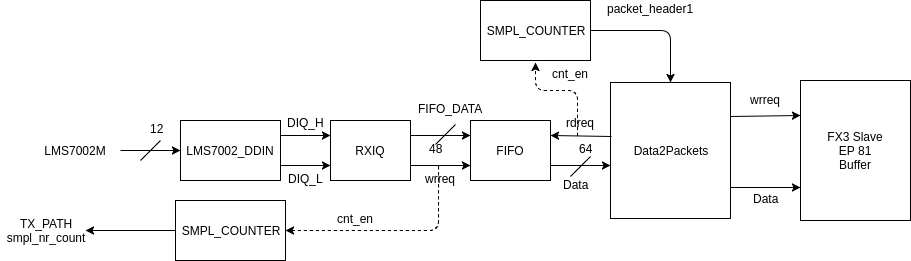
\includegraphics[width=\textwidth]{Figure/DATA2PACKETS.png}
\caption{LimeSDR FPGA RX Path}
\label{RX_Path}
\end{figure}

\paragraph{RX Path:}
\ac{VHDL} entities are primary level of \ac{RTL} abstraction, they define the hardware functionality in response to input signals.
\ac{VHDL} signals on the other hand, carry information from one entity to another.
This paragraph uses quoted text and italics to represent entities (blocks) and signals respectively.\\

Figure \ref{RX_Path} shows the overview of the RX Path implementation on the LimeSDR-USB \ac{FPGA}.
Sample data from the LMS7002M is captured by the "LMS7002\_DDIN", which uses an ALT DDIO IP block to capture in-phase and quadrature samples at double data rate.
This means that incoming data stream is latched both at the positive and negative edges of the clock.
"LMS7002\_DDIN" separates the sample data collected at the postive and negative edge into two different components: \textit{DIQ\_H} and \textit{DIQ\_L} repectively.
It introduces one clock delay between the input,LMS7002M Sample Stream, and the \textit{DIQ\_L}, \textit{DIQ\_H} outputs.\\

The "RXIQ" block is responsible for arranging the individual components into a single data stream of In-phase component of a sample followed by its Quadrature component.
It takes four component data coming from the "LMS7002\_DDIN" block and arranges arranges them into the sequence \textit{DIQ\_L},\textit{DIQ\_H}, \textit{DIQ\_L}, \textit{DIQ\_H}.
"RXIQ" takes one clock cycle for latching the inputs.
It takes three clock cycles for producing the structure.
Finally, the output is latched after one clock cycle from the internal output register.
It writes this structure every two clock cycles to the "FIFO" by enabling the \textit{wrreq} signal.
This means effectively one IQ sample is then sent to the "FIFO" every clock cycle. \\

The first "SMPL\_COUNTER" is a 64-bit counter which increases its count every time "RXIQ" asserts the \textit{wrreq} for writing new data samples to the "FIFO". 
The count is sent to the TX Path to track the number of produced samples. 
The second "SMPL\_COUNTER" is also a 64 bit counter which is enabled when the data is read from the "FIFO" by the "DATA2PACKETS" block.
It increases its count every clock cycle when the \textit{rdreq} signal is '1'.\\

The "FIFO" is implemented using the same read and write clocks, generated by the FPGA RX \ac{PLL}.
The read enable is controlled by the "RXIQ" using the \textit{wrreq} signal, so two new samples are written in two clock cycles of the RX PLL.
On the write side, the "DATA2PACKETS" controls the write enable signal (\textit{rdreq}).
The "FIFO" receives 48-bit data samples, stores it a \ac{FIFO} structure and keeps track of how many samples have been loaded into the \ac{FIFO}.
The "FIFO" takes one clock cycle for latching the input.
The counter for the number of elements is updated five clock cycles after the data has been latched.
\\

The "DATA2PACKETS" block is responsible for converting data samples into packets.
It mainly consists of two \ac{FSM}.
The first  \ac{FSM} controls the read and write signal for the input and output blocks.
It monitors the amount of data in the "FIFO", and when it is greater than the amount of data in one packet it asserts the \textit{rdreq} signal.
It takes two clock cycles for the "DATA2PACKETS" to register that the number of data elements in the "FIFO" is sufficient for one \ac{FPGA} packet.
The first \ac{FSM} takes two more clock cycles to generate the \textit{rdreq} signal after that.\\ 

The second \ac{FSM} arranges the data in the FPGA data packet structure (Figure \ref{trans_loop}).
It latches the value of the sample count from the second "SMPL\_COUNTER" when the first \ac{FSM} asserts the \textit{rdreq} signal.
It adds the sample count and different flags as meta-data for each \ac{FPGA} packet. 
Once, the first \ac{FSM} determines there is enough space to write the data in the FX3 buffer, it enables the \textit{wrreq} signal and writes 64 bits of data every clock cycle.
The second \ac{FSM} takes 6 clock cycles to output the first data element read from the "FIFO" after the \textit{rdreq} has been generated by the first \ac{FSM}.\\

\paragraph{RX Path Delays}
The delays introduced by the individual blocks has been highlighted in the previous paragraph.
\begin{itemize}
\item{Delay introduced by the "LMS7002\_DDDIN" block : 1 clock cycle}
\item{Delay introduced by the "RXIQ" block: 5 clock cycles ; 1 clock cycle each for input and output latching, and 3 clock cycles for the structure formation.}
\item{Delay introduced by the "FIFO" block: 6 clock cycles ; 1 clock cycle for input latching; 5 clock cycles for the increment of internal counter}
\item{Delay introduced the the "DATA2PACKETS" block: 10 clock cycles ; 4 clock for generation of \textit{rdreq} signal and 6 clock cycles for output of the first data element read from the "FIFO"}
\end{itemize}

The report will refer to these block delays as constant delays.
The constant delay is 22 clock cycles for even index samples, and 21 clock cycles for odd index samples. It can be summarized as:\\

\begin{subequations} \label{eq1}
\begin{align}
	sampl_{rel} = sampl_{abs} \ mod \ N \label{eq1.1}\\ 
  packet\_number= \floor*{\frac{sampl_{abs}}{N}} \label{eq1.2}\\
  \Delta_{constant} = \frac{22 - \floor*{sampl_{rel} \ mod \ 2 }}{f_s} \label{eq1.3}
\end{align}
  
\end{subequations}

N = Number of samples in one packet; N= even, $f_s$ is the \ac{FPGA} RX PLL frequency, $sampl_{rel}$ is the relative sample index and $sampl_{abs}$ is the absolute sample index in Equation \ref{eq1}

For example, with N=1020, $sampl_{abs}$ = 8000, packet\_number would be $\floor*{\frac{8000}{1020}} = 7$, and $sampl_{rel}$ would be  $8000 \ mod \ 1020 = 860$. \\
 
In addition to the constant delays, there are two more delays that need to considered.
They are Queuing Delay and the Streaming Delay.
The data elements in the "FIFO" has to wait until there is sufficient data for a single packet.
This waiting time is being referred to as Queuing Delay.
The Queuing Delay is dependent on the absolute sample number.
If the element is the $N^{th}$ sample, it has to wait for N clock cycles, where N is the number of samples in one packet.
If the element is the $N-1^{th}$ sample, it needs to wait only for one more cycle, that is two clock cycles.

\begin{equation} \label{eq2}
\Delta_{queuing} = \frac{N - 2 \times \floor*{\frac{sampl_{rel}}{2}}}{f_s}
\end{equation}

In Equation \ref{eq2}, N = Number of samples in one packet, $f_s$ is the \ac{FPGA} RX PLL frequency, and $samp_{rel}$ is defined by equation \ref{eq1.1}. \\

The "DATA2PACKETS" block outputs two samples in one clock cycle, hence the data will be streamed out sequentially.
The time a element has to wait to be streamed is being referred as the streaming delay.
The streaming delay is also dependent on the arrival time of the sample which is equivalent to the absolute sample number.
If the element is the $N^{th}$ sample, it is the first data element of a packet, it doesn't need to wait for any sample to be streamed ahead of it, so it has zero streaming delay.
On the other hand, the $N-1^{th}$ sample needs to wait for N-3 samples to streamed first, before it is outputted together with the $N-2^{th}$ sample.

\begin{equation}\label{eq3}
\Delta_{streaming} =\frac{\floor*{\frac{sampl_{rel}}{2}}}{f_s}
\end{equation} 
In Equation \ref{eq3}, N = Number of samples in one packet,  $f_s$ is the \ac{FPGA} RX PLL frequency, and $samp_{rel}$ is defined by equation \ref{eq1.1}. \\

The total delay can be calculated as :\\
\begin{subequations}\label{eq4}
\begin{align}
\Delta_{total}= \Delta_{constant} + \Delta_{queuing} + \Delta_{streaming} \\
\Delta_{total}= \frac{22 +  N - \floor*{\frac{sampl_{rel}}{2}} - \floor*{sampl_{rel} \ mod \ 2}}{f_s}
\end{align}
\end{subequations}



\subsubsection{Cypress EZ-FX3}
LimeSDR-USB uses a Cypress EZ-FX3 as \ac{USB} 3.0 peripheral controller.
It has a fully configurable, general programmable interface called the \ac{GPIF} II which allows integration with any processor like \ac{ASIC}, \ac{FPGA}, Image Sensors etc.
It also provides low speed interfaces like \ac{I2C}, \ac{SPI} for the low-speed \ac{IO} operations.\\

\begin{figure}[h!]
\centering
\hspace*{2.5cm}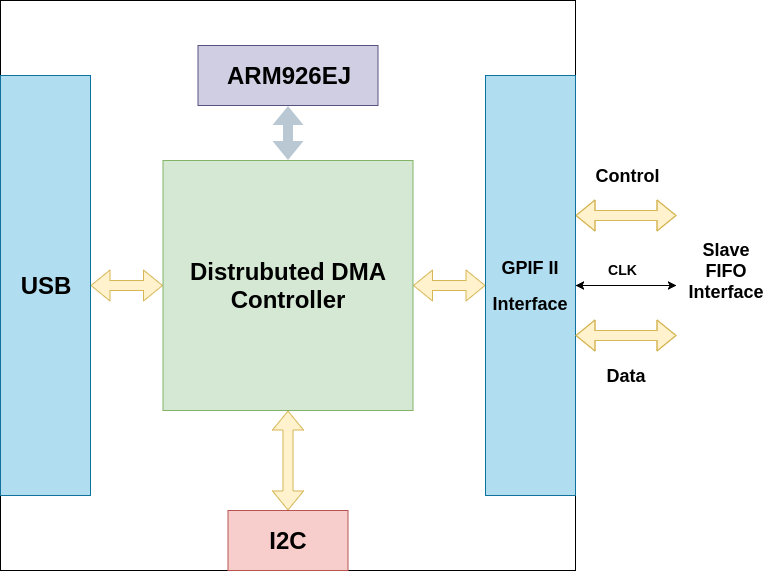
\includegraphics[width=0.8\textwidth]{Figure/FX3.png}
\caption{EZ-FX3 architecture}
\label{FX3_arch}
\end{figure}
The hardware architecture of EZ-FX3 is shown in Figure \ref{FX3_arch}.
The "ARM926EJ" is a 32-bit microprocessor operating at 200 MHz.
It is responssible for the configuring and controlling the distributed \ac{DMA} controller and the peripherals.
The "USB" block is a \ac{USB} 3.0 peripheral controller.
It implements the \ac{USB} 3.0 Physical Layer, and is responsible for handling the communication with the Host Computer.
The "\ac{GPIF} interface" block handles the data streams to and from the \ac{FPGA} of the LimeSDR-USB. 
It implements a Synchronous Slave FIFO Interface which is controlled by "Slave FIFO" block of the LimeSDR \ac{FPGA}.\\

For the purpose of this project, the implementation details for the USB and GPIF II interface needs to be explored further.
The next two paragraphs, concentrates on presenting the concrete understanding of these two important interface in the context of LimeSDR-USB.

\paragraph{LimeSDR USB endpoints}
\ac{USB} endpoint are buffers on the \ac{USB} device.
They are logical abstraction for having multiple parallel data streams use a single physical channel.
The LimeSDR-USB uses four different endpoints for the USB data transfer, these endpoints are divided into control and data endpoints for both the input and output directions.
The control endpoints are used for configuring and retrieving data from the LMS7002M, whereas data endpoints are used for streaming data to and from the LMS7002M data converters through the \ac{FPGA}.
The different endpoint address and their associated function in LimeSDR-USB is shown in Table \ref{Lime-USB_ep}\\

\begin{table}[h!]
\centering
\begin{tabular}{|c|c|}
\hline
Endpoint address & Function\\
\hline
0x01 & Stream Data Output\\
0x81 & Stream Data Input\\
0x0F & Control Data Output\\
0x8F & Control Data Input\\
\hline
\end{tabular}
\caption{LimeSDR USB transfer endpoints}
\label{Lime-USB_ep}
\end{table}

The \ac{USB} protocol specifies different transfers mechanisms depending on the requirement of the reliability and deterministic transfers.
Bulk Transfers are used for large bursty data.
They don't have any guarantees on the bandwidth and are transmitted when there is bandwidth available after other types of transfers.
They offer guaranteed delivery of data.\\

The LimeSDR-USB uses Bulk Transfers for the control transfers.
It sends bursts of data which are moved in the endpoint buffer of the Host Computer USB Controller which transfers it to the endpoint point buffer of the "USB" block shown in Figure \ref{FX3_arch}.\\

For the data transfers, the LimeSDR-USB uses bulk streams.
USB 3.0 protocol introduced stream pipes where a single \ac{USB} endpoint can be allocated to multiple data streams.
Each stream endpoint has their associated Stream ID which is used for tagging the data in the USB endpoint buffer.
Each of the data packets in the endpoint buffer are transmitted as a regular bulk transfer and the USB Controller on the other end decodes the Stream ID and sends it to the appropriate Stream endpoint. \\

USB endpoints also specifies the size of the data packet.
For USB 3.0 the maximum data packet size is 1024 bytes.
If the data sent to the USB Controller is greater than that, it segments that into multiple data packets and sends them as multiple bursts of data in a single USB Transaction. 
 
\paragraph{GPIF II}
The \ac{GPIF} II is a programmable state machine, that provides the flexibility of implementing a custom interface.
The GPIF II segments the functionality into control and data intefaces.
For the data interface, the LimeSDR-USB defines a 32-bit interface running at 100 MHz.
The state transitions of the state machine are based on the input control signals from the GPIF II interface.
The output control signals are driven by the state transitions of the internal state machine.\\

LimeSDR-USB implements a Slave FIFO interface using the \ac{GPIF} II interface.
The Slave FIFO interface allows the \ac{FPGA} to perform read/ write operations on the EZ-FX3 internal FIFO buffers directly.
The control interface is used for addressing the FX3 FIFOs and signaling read and write operations.
In addition, the control interface has flag signals to indicate events to the FIFO Slave Interface.
The 32-bit data interface transfers the data according to the signaling and addressing used on the control interface.\\

The distributed \ac{DMA} controller uses sockets and threads for allowing data transfer between the FX3 RAM and the peripherals.
They are explained in the next paragraph to help understand the Slave FIFO interface in details.

\paragraph{Sockets and Threads}
Sockets are connections between a FX3 peripheral like GPIF II, I2C and FX3 RAM. 
The FX3 microprocessor initializes \ac{DMA} buffers, which are used for intermediate storage of data transferred through the FX3.
The microprocessor keeps the address and size of these \ac{DMA} buffers in a linked list like structure.
The elements of this structure are referred to as \ac{DMA} descriptor.
The sockets are implemented as a structure with a pointer to a \ac{DMA} descriptor and interrupt flags.\\ 

The sockets can signal other sockets automatically without CPU intervention or signal the CPU through interrupts.
Automatic signaling is used when the FX3 CPU does not need to modify any data in the data stream.
The socket which is writing data to the buffer is called producer socket and the socket reading data from the buffer is called consumer socket according to the terminology defined by (refer document.)\\

One producer socket and one consumer socket accessing the same \ac{DMA} buffer can be encapsulated in a configuration referred to as \ac{DMA} channel.
The \ac{DMA} channel can have multiple \ac{DMA} buffers.
Each DMA buffer has its own empty/full flag to signal the producer and consumer sockets.
For example, if a 1024 bytes socket is allocated to the DMA channel, when the producer sockets write 1024 bytes, the full flag will be enabled.
In case of LimeSDR-USB, two \ac{DMA} channels are defined: TX \ac{DMA} channel and RX \ac{DMA} channel, with a GPIF II socket and USB socket as producer and consumer sockets.
Each of channel have multiple \ac{DMA} buffers, and each buffer is allocated 4096 bytes.\\

The sockets are internal to the FX3, so for external devices to access the \ac{DMA} buffers, GPIF threads are defined.
They connect sockets with external pins, like for Slave FIFO interface, they connect the GPIF II interface with GPIF II sockets.\\


\subsection{LimeSDR USB Software Architecture.}

In this subsection, the report explains the driver of the LimeSDR-USB.
The software architecture of the LimeSDR-USB is shown in Figure \ref{Lime_Software}.\\

\begin{figure}[h!]
\centering
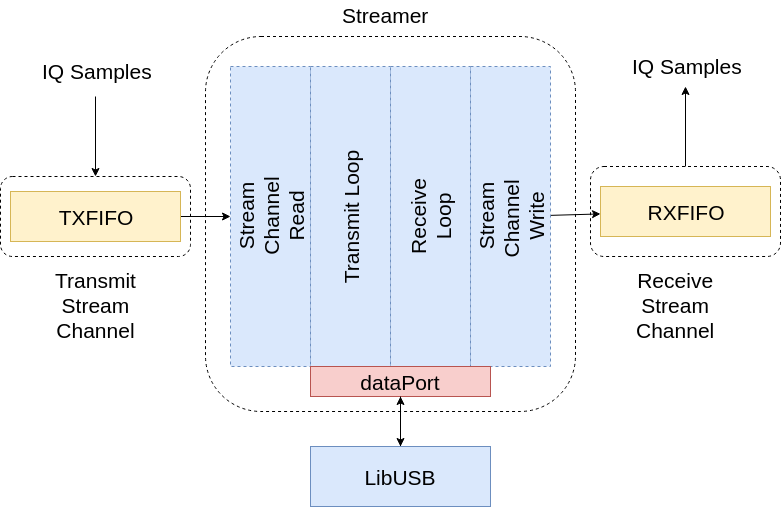
\includegraphics[width=0.8\textwidth]{Figure/Lime_Software.png}
\caption{LimeSDR USB software architecture}
\label{Lime_Software}
\end{figure}

The "Streamer" block is the main software component responsible for interacting with the LimeSDR-USB.
LimeSDR defines "dataPort" as an abstract interface, whose methods can be mapped to one specific interface implementation like \ac{PCIe} or USB depending on the configuration defined by the "Streamer" block.
In case of LimeSDR-USB, the dataPort is configured to use \ac{USB} bus.
For interacting with application software like GNU Radio "Stream Channels" are defined.
They are basically FIFO's with control logic for receiving or sending data from the application software.
To understand the functionality of the "Streamer" block, let's take a look at the TX data path.
The RX Path is vice-versa of the TX Path.\\

\paragraph{TX Data Path} \label{TX Data Path} The application software configures the TX Stream Channels through the Lime \ac{API}. 
Then the TX FIFO's are initialized and the control parameter like batchsize( shown in Figure \ref{trans_loop}) of the \ac{FPGA} packets and the data format for the data to be stored in the FIFO is sent to the "Streamer".
The Streamer parses these information and configures the hardware data path with the provided configuration.
The "Streamer Transmit Loop" initalizes internal buffers which are used for sending data through the "dataPort".\\
\begin{figure}[h!]
\centering
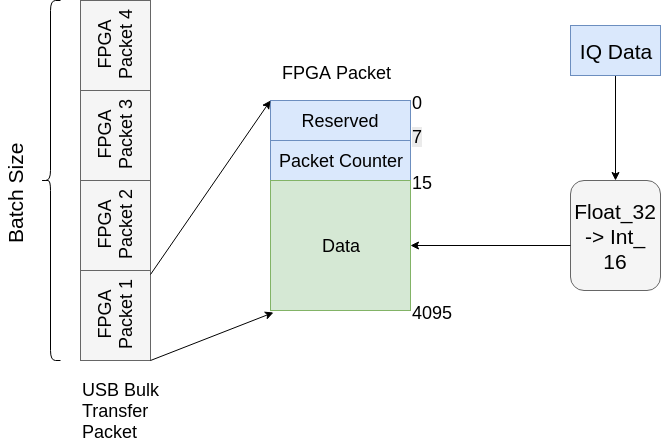
\includegraphics[width=0.8\textwidth]{Figure/DriverHost.png}
\caption{Streamer Transmit Loop}
\label{trans_loop}
\end{figure}
 
The application software pushes data to the TX "Stream Channel" shown as "IQ Data" in Figure \ref{trans_loop}.
The "Streamer Transmit Loop" runs continuously and once there is data in the "Stream Channel" FIFOs it reads the data using the "Stream Channel Read" function.
It converts the data, for example from 32-bit float data to 16 bit integer data, and copies the data to its internal buffers.
It then packs the data into a FPGA data packet format shown as the middle component of Figure \ref{trans_loop}.
Each \ac{FPGA} data packet contains flags and packet counter field followed by  4080 bytes of data.
These \ac{FPGA} data packets are batched together as specified by the batchsize.
This batch is sent to the USB Host Controller to be transmitted to the LimeSDR-USB using libusb.

\paragraph{TX Control Path} The LimeSDR-USB is configured at initialization using the lms7 \ac{API}.
The lms7 \ac{API} provides an abstraction layer for configuring the LimeSDR-USB.
It provides the means to control the LMS7002M, Si5351 clock controller through the NIOS SPI interface.
The lms7 API packs the control data into LMS64 control packets shown in figure \ref{lms_packet}.
One LMS64C protocol packet (Figure \ref{lms_packet}) is maximum 64 bytes.
If the data to be sent is larger than that the data field is segmented into several packets.
The "LMS64C\_Protocol" keeps a packet buffer and adds the prepared packet to this buffer.
These packets are then sent to the "connectionFX3" module which writes it to the control endpoint using the "dataPort".



\begin{figure}[h!]
\centering
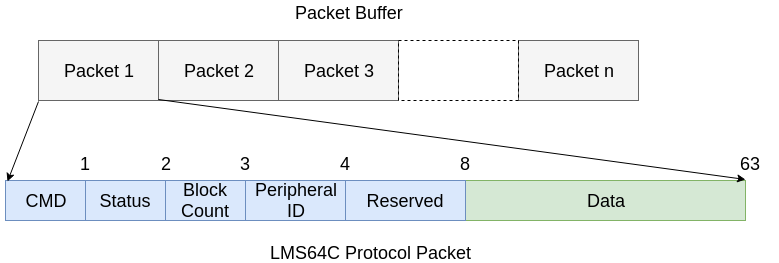
\includegraphics[width=\textwidth]{Figure/LMS64C_Packet.png}
\caption{LMS Control Packet Structure}
\label{lms_packet}
\end{figure}

\section{Wime Project}
Wime Project was created with the objective of providing experimentation as a wireless communication system performance evaluation tool.
The project focuses on evaluation of physical layer strategies using USRP \ac{sdr} platform.
It provides a 802.15.4 testbed which is inter-operable with the the off-the shelf TelosB nodes running the Contiki operating system.

\subsection{IEEE 802.15.4}
The IEEE 802.15.4 is a \ac{LR-WPAN} specification aiming to be a ultra low-complexity, ultra-low power and low datarate specification.
It specifies the \ac{PHY} and \ac{mac} for \ac{LR-WPAN}s.
It forms the basis for network protocols like \ac{6LoWPAN}, Zigbee, WirelessHart.
It is intended to provide a data-rate of 250 kbps at 10 meters communication range.\\

The IEEE 802.15.4 network topologies provide ways in which devices can talk to different nodes in the network.
The main two network topologies used in IEEE 802.15.4 are: star and mesh.
In star all the devices communicate to one another through the central device called the \ac{PAN} coordinator.
In mesh, the devices can talk to one another without the need for a central coordinator.\\

These network topologies helps in defining the role and type of device.
\ac{RFD} can communicate without routing functionality so they usually are the end devices in a network.
\ac{FFD} can route information in addition to regular communication.
Coordinator is a special \ac{FFD} which sets up the network and acts as the manager of the network.\\

The IEEE 802.15.4 \ac{PHY} specifies defines different radio channels and modulation techniques for these network nodes.
It specifies \ac{O-QPSK}, \ac{BPSK}, \ac{ASK}, \ac{CSS} etc. as physical layer modulation techniques.
The main frequency band of interest is ISM band at 2.4 GHz where 20  channels are available globally.
The channels are spaced at 5 MHz, having channel bandwidth of 2 MHz.\\

The \ac{mac} layer offers handshake for reliability.
\ac{csma} with collision avoidance, \ac{tdma} with synchronization beacons and \ac{GTS} are defined as methods of medium access.
There are four different \ac{mac} frames defined for different unique functions: Data, Acknowledgement, Beacon and MAC Command.
Data and Acknowledgment frames are used for data communication, whereas Beacon and \ac{mac} command are used for network maintenance.\\

\begin{figure}[h!]
\centering
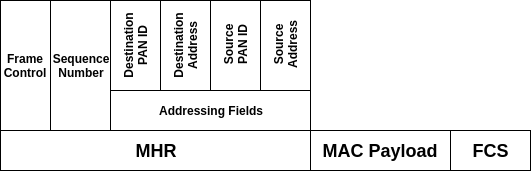
\includegraphics[scale=0.6]{Figure/DataFrame.png}
\caption{MAC Data Frame Structure}
\label{data_frame}
\end{figure}

The relevant \ac{mac} data frame structure has been shown in Figure \ref{data_frame}.
The function of each field is described below:
\begin{itemize}
\item{\textbf{MHR} defines the MAC data frame header. It consists of the following subfields:
\begin{itemize}
\item{\textbf{Frame Control} specifies the type of the frame and how the rest of frame is structured like the source and destination addressing modes.}
\item{\textbf{Sequence Number} specifies the sequence identifier for the frame}
\item{\textbf{Destination PAN ID} is an unsigned integer which is the unique \ac{PAN} ID for the destination node.}
\item{\textbf{Destination Address} is the \ac{mac} address of the intended recipient.}
\item{\textbf{Source PAN ID} is the \ac{PAN} ID of the sender.}
\item{ \textbf{Source Address} is the \ac{mac} address of the originator of the frame.} 
\end{itemize}}
\item{\textbf{MAC Payload} is the link layer frame which includes the data payload. }
\item{\textbf{\ac{FCS}} is a 16-bit ITU-T \ac{CRC} calculated over the MHR and MAC Payload fields.} 
\end{itemize}


Since, \ac{O-QPSK} modulation is being used in the Wime project, the next paragraph elaborates on the \ac{O-QPSK} modulation.

\paragraph{\ac{O-QPSK}}

The O-QPSK PHY specifies the PHY Data Packet as shown in Figure \ref{OQPSK_packet}.

\begin{figure}[h!]
\centering
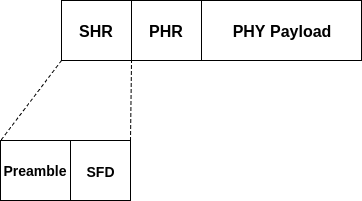
\includegraphics[scale=0.6]{Figure/OQPSK.png}
\caption{O-QPSK PHY Packet}
\label{OQPSK_packet}
\end{figure}

\begin{itemize}
\item{ \textbf{\ac{SHR}} is used for indicating the start of the frame. 
It is composed of two sub subfields : Preamble and \ac{SFD}.
For the O-QPSK, the preamble is four bytes with decimal value of "0000".
The SFD is one byte long as is formatted as "A7" in hexadecimal.}
\item{ \textbf{PHR} is the header for the physical layer packet and it specifies the frame length.}
\item{ \textbf{PHY Payload} is the data payload, which for the purpose of this project is the MAC data frame.
The PHY payload has a maximum size of 127 bytes.}
\end{itemize}
 

O-QPSK PHY uses 16-ary quasi orthogonal modulation.
The data packet is converted to data symbols, the symbols subsequently are converted to chips, which are modulated onto the carrier signal.
The octets of the PHY data packets are converted into symbols starting from the Preamble and ending with the last octet of the PHY Payload.
The least significant bits of an octet is mapped to one symbol and the most significant bits mapped to another symbol.\\

Each symbol is mapped to a 32-bit \ac{PN} sequence, which are related to each other through cyclic shifts and/or conjugation.
The even indexes of the chip sequence are modulated onto the In-Phase component of the carrier as shown in Figure \ref{IQ_TC}.
On the other hand, the odd indexes of the chip sequences are modulated onto the Quadrature component of the carrier.
The chips are represented by a half-sine pulse shape shown in equation \ref{eq5}

\begin{equation}\label{eq5}
p(t) = 
\begin{cases} 
   sin( pi \times \frac{t}{2T_c})  \ ,0 \geq t \leq 2T_c \\
   0    \ ,otherwise
  \end{cases}
\end{equation}
$2T_c$ is the period of the half sine wave pulse in equation \ref{eq5}.
The quadrature component is delayed by $T_c$ as shown in Figure \ref{IQ_TC}.

\begin{figure}[h!]
\centering
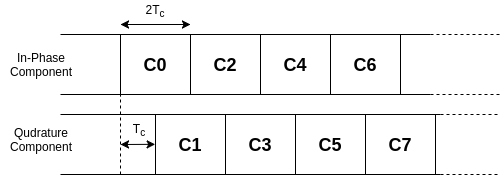
\includegraphics[scale=0.6]{Figure/IQ_TC.png}
\caption{In-Phase and Quadrature Chip Sequences}
\label{IQ_TC}
\end{figure}

\subsection{Wime Project GNU Radio Implementation}
Wime Project is build on the UCLA 802.15.4 PHY implementation designed  by Thomas Schmid.
It ports the existing implementation to the modern GNU Radio software framework.
It furthermore extends the PHY implementation with a \ac{mac} layer and adds Rime Stack as a network layer.
The implementation details of the PHY layer and the MAC layer is described below.\\

\begin{itemize}

\item{\textbf{Modulation} The Wime \ac{mac} works with asynchronous mesages, whereas the \ac{PHY} is implemented with stream interfaces.
The GNU Radio modulation flow graph is shown in Figure \ref{TX flow graph}.
At first, these asynchronous \ac{mac} messages are converted to a tagged stream by the "PDU to Tagged Stream block".
\begin{figure}[h!]
\centering
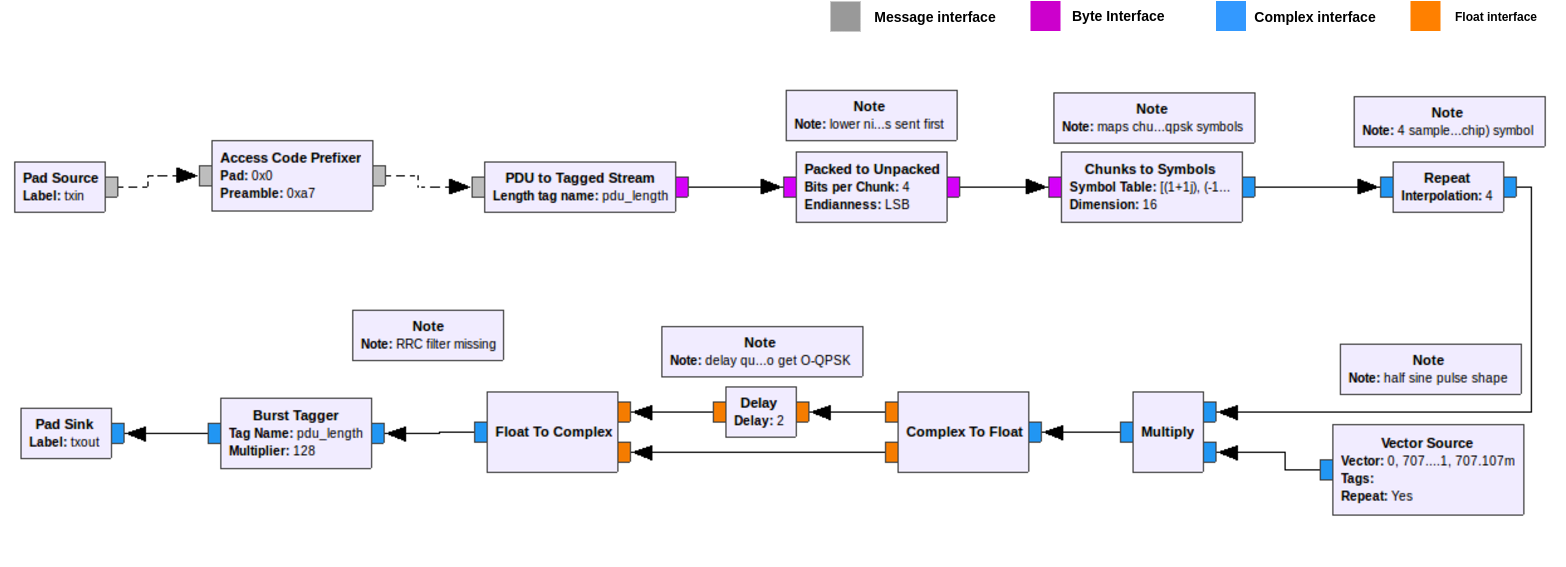
\includegraphics[width=0.8\textwidth]{Figure/TXPath.png}
\caption{GNU Radio Modulation flow graph}
\label{TX flow graph}
\end{figure}

The individual octets of the stream are then converted to symbols as described previously in the \ac{O-QPSK} paragraph by the "Packed to Unpacked Block".
Instead of converting the symbols to chips directly and then segmenting into In-Phase and Quadrature components as in UCLA PHY.
Wime Project implementation directly converts a symbol through a symbol table directly into a sequence of complex in-phase and quadrature values.
Each symbol input results in 16 complex chips.
These individual chips are interpolated by repeating a single chip four times by the "Repeat" block.
The repeated chips are then multiplied with a sine function at different phases, differing by $\pi/4$.
This process makes a single chip to be four samples wide.
The quadrature component is delayed by two samples to satisfy the offset requirement ($T_c$).}

\begin{figure}[h!]
\centering
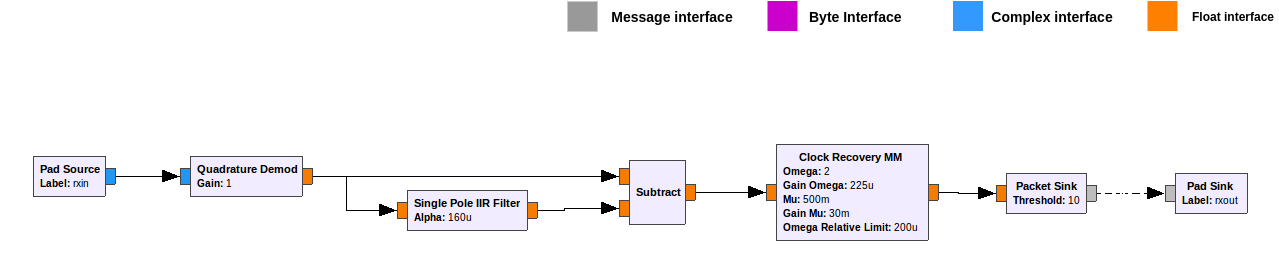
\includegraphics[width=0.8\textwidth]{Figure/RXPath.png}
\caption{GNU Radio Demodulation flow graph}
\label{RX flow graph}
\end{figure}


\item{\textbf{Demodulation} The data stream from the USRP is passed through a "Quadrature Demodulation" block as shown in Figure \ref{RX flow graph}.
It does FM demodulation of the received signal stream.
"Clock Recovery" module takes this demodulated signal stream and performs  decimation first, followed by  Mueller and Müller discrete-time error-tracking synchronizer.
The "Clock Recovery" block outputs the chip sequences obtained from the incoming signal stream.
These chip sequences are then sliced and converted to symbols by the "Packet Sink" block.
The decoded valid message is then outputted to the Wime \ac{mac}.}

\item{\textbf{MAC} The Wime Project adds a very simple MAC which encapsulates upper layer packets with the MAC header and adds the \ac{FCS}.
When receiving messages from the \ac{PHY}, it does a validity check on the received message.
On successful validation of the received message, it strips away the \ac{mac} header.
The \ac{mac} layer transmits the message immediately without any carrier sensing.}
\end{itemize}

\section{Tools Used}
\subsection{USBMon}
It is kernel facility provided to collect I/O traces on the USB Bus\cite{_usbmon}. USBMon reports the requests made to and by the USB Host Controller Drivers(HCD). It provides two kinds of API's : binary and character. The binary API is accessed by character devices located in the /dev namespace. The character API provides human readability and uniform format for the traces.The kernel data from the USBMon text data is made available to the userspace using debugfs\cite{_debugfs} utility.

\begin{figure}[h!]
\centering
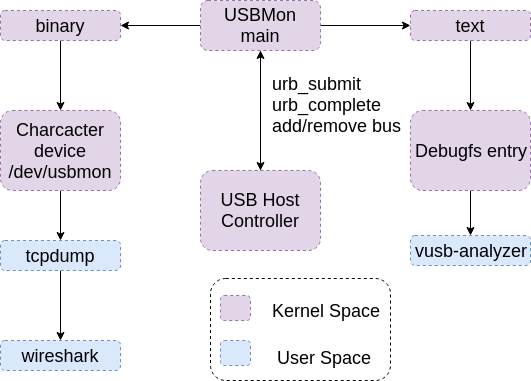
\includegraphics[width=\textwidth]{Figure/USBMon.png}
\caption{USBMon Architecture(Adapted from \cite{basak_usb_2018}).}
\end{figure}

\subsubsection{Text Data Format}
\begin{table}[h!]
\centering
\begin{tabular}{|c|c|c|c|c|}
\hline
URB Tag & Timestamp & Event Type & Address & URB Status\\
\hline
ffff8fbdbbae4000 & 2942307806 & S & Bo:3:008:15 & -115\\ 
\hline
\end{tabular}
\begin{tabular}{|c|c|c|}
\hline
Data Length & Data Tag & Data\\
\hline
64 & = & 21000100 00000000 002a0484 00000000 000000\\
\hline
\end{tabular}
\caption{Text USB Trace Example.}
\end{table}

\begin{itemize}
\item {\textbf{URB Tag:} URB Identification number, it is usually the in kernel adress of the URB structure.}
\item{\textbf{Timestamp:} The timestamp for the URB event at the HCD in microseconds. It is measured by the usbmon main utility using \textit{gettimeofday()} function of \textit{time.h}.}
\item{\textbf{Event Type:} It specifies the event type of the HCD event. S - Submission C -Complete E - submission error.}
\item{\textbf{Address: } It consists of four fields separated by colons. The URB type and direction, bus number, device number, endpoint number. The URB type and direction specifies the type of USB transfer(can be both synchronous and asynchronous).\\
\begin{table}[h!]
\centering
\begin{tabular}{|c|c|c|}
\hline
Bi & Bo & Bulk Input and Output.\\
Ci & Co & Control Input and Output.\\
Ii & Io & Interrupt Input and Output.\\
Zi & Zo & Isochronous Input and Output.\\
\hline
\end{tabular}
\caption{URB Type and Direction.}
\end{table}\\
The USB device transfers data through a pipe to a memory buffer on the host and endpoint on the device. The type of data transfer depends on the endpoint and the requirements of the function. The transfer types are as follows\cite{_usb_data_transfer}:

\begin{itemize}
\item{\textbf{Control Transfers:} It is mainly used for configuration, command and status operations.}
\item{\textbf{Bulk Transfers:} Bulk Transfer are used for bulky,non-periodic non time-sensitive burst transmissions.}
\item{\textbf{Interrupt Transfers:} It is used for mainly sending small amounts of data infrequently or asynchronously.}
\item{\textbf{Isochronous Transfers:} Isochronous transfers are mainly used for periodic, continuous streams of time sensitive data.} 
\end{itemize}
%USB endpoint as explained by \cite{_usb_endpoint} , refers to the buffers on the USB device. The host computer irrespective of the host operating system can communicate by reading and writing to these buffers. They can be data endpoints and control endpoints.Data endpoints are used for transferring data whereas the control endpoint is used for configuration and device specific control.
}

\item{\textbf{Data Length:} For urb\_submit it gives the requested data length and for callbacks it is the actual data length.}

\item{\textbf{Data tag:} If this field is '=' then data words are present.}

\item{\textbf{Data:} The data words contains in the USB transfer packet.}
\end{itemize}

\subsubsection{Raw Binary}
The overall data format is same as the text data, the data is available in raw binary by accessing character devices at /dev/usbmonX. The data can be read by using \textit{read} with \textit{ioctl} or by mapping the buffer using \textit{mmap}. The usbmon events are buffered in the following format:

\begingroup
\centering\scriptsize\begin{lstlisting}
struct usbmon_packet {
	u64 id;			/*  0: URB ID - from submission to callback */
	unsigned char type;	/*  8: Same as text; extensible. */
	unsigned char xfer_type; /*    ISO (0), Intr, Control, Bulk (3) */
	unsigned char epnum;	/*     Endpoint number and transfer direction */
	unsigned char devnum;	/*     Device address */
	u16 busnum;		/* 12: Bus number */
	char flag_setup;	/* 14: Same as text */
	char flag_data;		/* 15: Same as text; Binary zero is OK. */
	s64 ts_sec;		/* 16: gettimeofday */
	s32 ts_usec;		/* 24: gettimeofday */
	int status;		/* 28: */
	unsigned int length;	/* 32: Length of data (submitted or actual) */
	unsigned int len_cap;	/* 36: Delivered length */
	union {			/* 40: */
		unsigned char setup[SETUP_LEN];	/* Only for Control S-type */
		struct iso_rec {		/* Only for ISO */
			int error_count;
			int numdesc;
		} iso;
	} s;
	int interval;		/* 48: Only for Interrupt and ISO */
	int start_frame;	/* 52: For ISO */
	unsigned int xfer_flags; /* 56: copy of URB's transfer_flags */
	unsigned int ndesc;	/* 60: Actual number of ISO descriptors */
};	
\end{lstlisting}
\endgroup


\subsection{pidstat}
Pidstat is a Linux tool provided the sysstat package.
It can be used to monitor the resource usage of a Linux process/processes.
It can be configured to collect information on CPU utilization, memory utilization, context switches and the time  used by the process at application level and the time used in kernel level.
It collects the information at one second intervals and the time duration for one collection can be specified during the process invocation.

